\documentclass[10pt]{article}
\usepackage[margin=0.78in]{geometry}
\usepackage[T1]{fontenc}
\usepackage{lmodern,microtype,booktabs,graphicx,xcolor,hyperref,placeins}
\definecolor{navy}{HTML}{16324F}\definecolor{teal}{HTML}{087E8B}
\hypersetup{colorlinks=true,linkcolor=navy,urlcolor=teal}
\title{\textcolor{navy}{A Stronger Drift Baseline}\[3pt]
\large ADWIN with Delayed, Budgeted Prediction-Error Feedback}
\author{23I-2581 and 23I-2604\\Data Analysis and Visualization --- Phase 3 addendum}
\date{17 November 2026}
\begin{document}\maketitle
\begin{abstract}
We add River's canonical ADWIN detector as a supervised baseline on the exact same frozen predictions, 30 evaluation seeds, seven synthetic conditions, audit cohorts, budgets and label delays used in the policy matrix. ADWIN receives row-level binary prediction errors only from sampled cohorts after their labels are released. The comparison demonstrates that detector choice is constrained by the feedback schedule: under strict caps, a single bootstrap cohort supplies no second labeled sample from which to detect a change. This is a scoped baseline evaluation, not a claim of ADWIN's general performance.
\end{abstract}
\section{Method and timing}
We use River 0.27.0's implementation of ADWIN/ADWIN2. Its significance value is $\delta=0.002$, the documented default. We set \texttt{clock=1} so checks occur after each received error; the documented defaults for maximum buckets (5), minimum subwindow length (5) and grace period (10) are retained. River describes ADWIN as comparing the means of two subwindows in an adaptive window; see the [\href{https://riverml.xyz/latest/api/drift/ADWIN/}{River ADWIN API}]. The underlying method is due to Bifet and Gavald\`a~\cite{bifet2007}.

The detector receives a zero/one error sequence from the 500 rows in each selected audit cohort, in row order. It receives nothing from unselected batches. A selected source batch $s$ is first ingested at decision clock $t$ only when $s+d<t$. A fixed initial probe at $\lceil24/B\rceil$ is shared with the released-error policy. A new audit is requested when ADWIN signals and the strict budget has room; exact-quota mode fills unused quota at the end and marks those forced acquisitions. Each clock predicts before its current batch's labels can be used.

ADWIN is a supervised error-change detector; it does not detect feature-only drift without labels. Uncertainty resamples the 30 seeds after averaging the seven matched conditions and three budget levels. Neither conditions nor batches are treated as independent replicates.
\section{Results}
\begin{figure}[ht]
\centering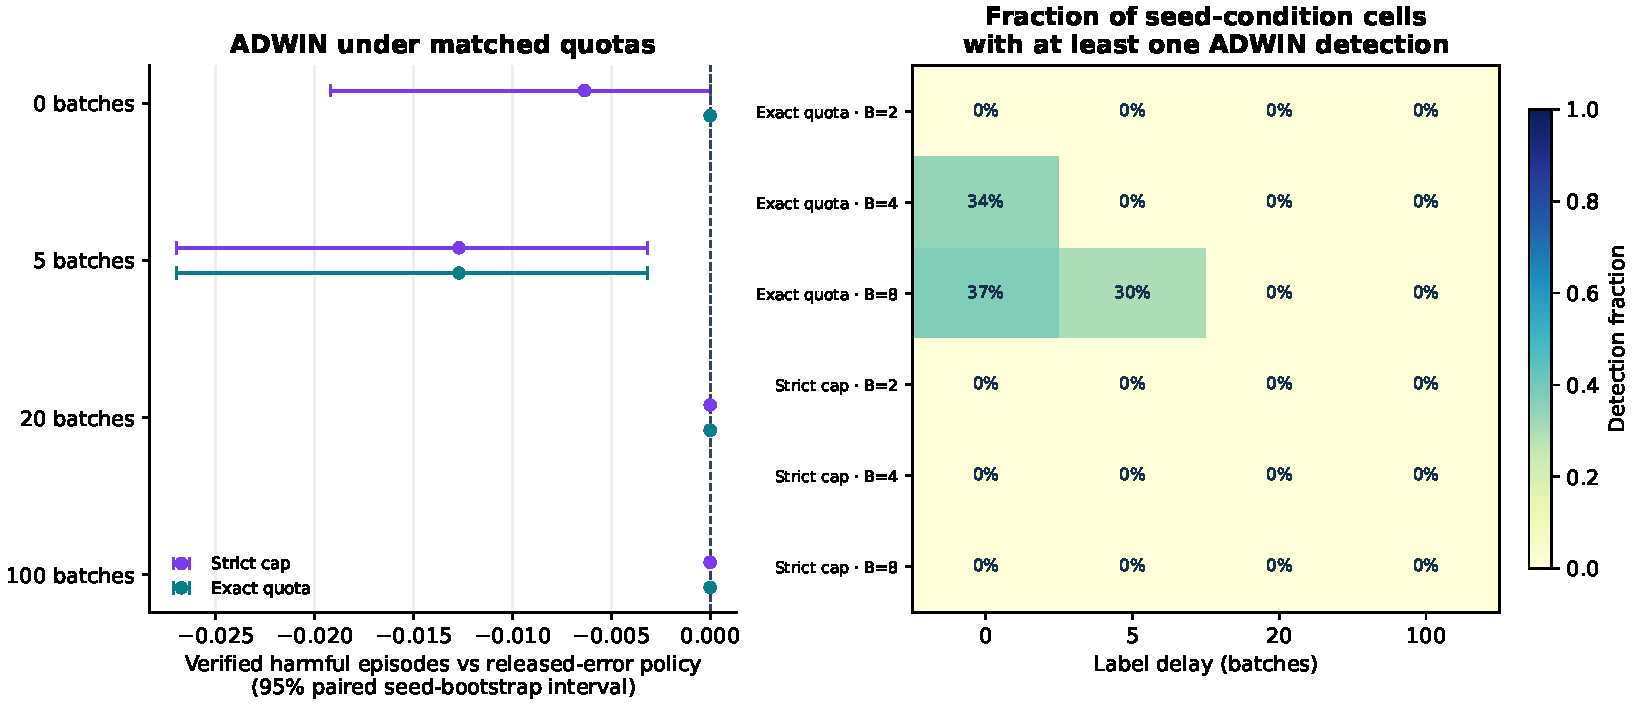
\includegraphics[width=\linewidth]{adwin_effects.pdf}
\caption{Left: paired ADWIN-minus-released-error differences in harmful episodes verified by stream end; seed-bootstrap intervals average over matched conditions and budgets. Right: proportion of seed-condition cells with at least one ADWIN event. A detector event is not itself evidence that harmful performance was correctly identified.}
\end{figure}
\begin{table}[ht]
\centering\small\begin{tabular}{@{}llrrrr@{}}\toprule
Cost mode & Delay & Audits & Error rows ingested & Detection cells & Verified episodes\\\midrule
Exact quota & 0 & 4.67 & 1833 & 149/630 & 0.513 \\
Exact quota & 5 & 4.67 & 667 & 63/630 & 0.324 \\
Exact quota & 20 & 4.67 & 167 & 0/630 & 0.000 \\
Exact quota & 100 & 4.67 & 0 & 0/630 & 0.000 \\
Strict cap & 0 & 1.00 & 500 & 0/630 & 0.190 \\
Strict cap & 5 & 1.00 & 500 & 0/630 & 0.190 \\
Strict cap & 20 & 1.00 & 167 & 0/630 & 0.000 \\
Strict cap & 100 & 1.00 & 0 & 0/630 & 0.000 \\\bottomrule\end{tabular}
\caption{Descriptive averages across budgets, seeds and conditions. The event count is out of 210 seed-condition streams for each delay and cost mode.}
\end{table}
\FloatBarrier
\section{Interpretation and limitations}
ADWIN produced at least one event in 212 of 5,040 policy cells; all such cells were exact-quota runs. No strict-cap cell fired after its initial probe. This is a feedback deadlock in the declared strict-cap rule: after one sampled cohort ADWIN has no second selected cohort to compare, so it cannot trigger the next audit. Exact-quota tail acquisitions supply further data, but those acquisitions are mandated by budget completion and arrive late; their event counts are not an online detection success rate. At delays 20 and 100, the finite 24-batch horizon leaves little or no released feedback.

The exact-quota paired contrast against released-error is small in the reported aggregate; it does not show ADWIN is generally better or worse. The strict-cap comparison is also constrained by fewer audits. This implementation demonstrates that a named baseline can be faithfully placed inside the same delayed feedback contract and exposes how a bootstrap schedule affects detector viability. A future operational ADWIN policy needs a predeclared exploration schedule that yields at least two informative audited cohorts without exceeding the same budget; this would be a new policy and requires a separately locked evaluation.

All experiments reuse the cached synthetic predictions and truth from the locked evaluation. The detector is not tested on new seeds or natural streams. It does not estimate causal feature importance, calibration quality, analyst benefit, or monetary acquisition cost. River parameters are fixed and were not tuned on final seeds.
\section{Reproduction}
From the project root, install the declared dependencies, then run:
\begin{verbatim}
python scripts/run_adwin_audit_baseline.py
python scripts/report_adwin_audit_baseline.py
\end{verbatim}
The protocol lock records the River version, parameters, source hashes and output hashes. The editable report command compiles this TeX with Tectonic and hashes the resulting PDF.
\begin{thebibliography}{1}
\bibitem{bifet2007} A. Bifet and R. Gavald\`a, ``Learning from time-changing data with adaptive windowing,'' in \emph{Proc. 7th SIAM Int. Conf. on Data Mining}, 2007, pp. 443--448, doi: \href{https://doi.org/10.1137/1.9781611972771.42}{10.1137/1.9781611972771.42}.
\end{thebibliography}
\end{document}
